\documentclass[12pt]{article}
\usepackage{amsfonts}
\usepackage{mathrsfs}
\usepackage{booktabs}
\usepackage{graphicx}
\usepackage{subfigure}
%\usepackage{bbm}
\usepackage{color}
\usepackage{amsmath}
\usepackage{cases}
\usepackage{bbding}
\newcounter{mytempeqncnt}
\usepackage{amssymb}
\usepackage{makecell}
\usepackage{threeparttable}
\usepackage{booktabs}
\usepackage{multirow}
\newtheorem{theorem}{Theorem}
\newtheorem{proof}{Proof}

\pagestyle{empty} \textwidth 17cm \textheight 22.5cm
\renewcommand{\baselinestretch}{1.2}
\newcommand{\BOX}{\hfill $\Box$}
\newcommand{\NAB}{\hfill $\nabla \nabla \nabla$}
\newcommand{\BYDEF}{\stackrel{\rm \Delta}{=}}
\newcommand{\bm}[1]{\mbox{\boldmath{$#1$}}}
\topmargin -2.0cm \oddsidemargin 0.0cm \evensidemargin 0.0cm
\parskip 0.3cm
\parindent 0.0cm
\baselineskip 0.5cm \makeatletter
\def\EquationsBySection{\def\theequation{\thesection.\arabic{equation}}%
\@addtoreset{equation}{section}}
\def\TheoremsBySection{\def\thetheorem{\thesection.\arabic{theorem}}%
\@addtoreset{theorem}{section}}
\def\DefinitionsBySection{\def\thedefinition{\thesection.\arabic{definition}}%
\@addtoreset{definition}{section}}
\def\RemarksBySection{\def\theremark{\thesection.\arabic{remark}}%
\@addtoreset{remark}{section}}
\def\LemmasBySection{\def\thelemma{\thesection.\arabic{lemma}}%
\@addtoreset{lemma}{section}}
\def\AssumptionsBySection{\def\theassumption{\thesection.\arabic{assumption}}%
\@addtoreset{assumption}{section}} \makeatother
\newcommand{\ba}{\begin{array}}
\newcommand{\ea}{\end{array}}
\newcommand{\be}{\begin{equation}}
\newcommand{\ee}{\end{equation}}
\newcommand{\bea}{\begin{eqnarray}}
\newcommand{\eea}{\end{eqnarray}}
\newcommand{\bc}{\begin{center}}
\newcommand{\ec}{\end{center}}
\newcommand{\hs}{\hspace}
\newcommand{\vs}{\vspace}
\newcommand{\lt}{\left}
\newcommand{\rt}{\right}
\newcommand{\bib}{\bibitem}
\newcommand{\ds}{\displaystyle}
\newcommand{\fc}{\frac}
\newcommand{\nm}{\nonumber}
\newcommand{\ol}{\overline}
\newcommand{\da}{\Delta}
\newcommand\old[1]{}
\newtheorem{remark}{Remark}
\EquationsBySection \TheoremsBySection \DefinitionsBySection
\RemarksBySection \LemmasBySection \AssumptionsBySection
\begin{document}
\begin{flushright}
     Dr. Zhixin Liu \\
    Institute of Electrical Engineering\\
    Yanshan University \\
    Qinhuangdao, 066004 China  \\
    E-mail: lzxauto@ysu.edu.cn
    \\
    %\today
\end{flushright}
\begin{flushleft}
Prof. Tao Dusit Niyato\\
Editor, IEEE Transactions on Vehicular Technology



\end{flushleft}
Dear Editor,\\

Thank you very much for your email and the review comments on our paper:
\begin{center}
{\bf Ref.  Number VT-2021-01163}\\
{``Resource Allocation in D2D Enabled Vehicular Communications: A Robust Stackelberg Game Approach based on Price-Penalty Mechanism"}
\end{center}

As kindly suggested by you and the reviewers, the paper has been
seriously revised in accordance to the constructive and helpful
comments from you and the reviewers for improving the quality
further. All the modifications in the revision have been marked \textcolor{red}{in
red}. For more information, please see the detailed Responses to the
Reviewers.

We would like to express our sincere appreciation to you for your prompt and professional handling of our manuscript.

Looking forward to hearing from you.

Yours sincerely,

\vspace{3mm} Zhixin Liu


\newpage
\pagestyle{plain}
\title{\Huge{Responses to Reviewers\thanks{For the paper, Ref.  Number VT-2021-01163, ``Resource Allocation in D2D Enabled Vehicular Communications: A Robust Stackelberg Game Approach based on Price-Penalty Mechanism," submitted to {\em IEEE Transactions on Vehicular Technology}.}}}
\author{}
\date{}
\maketitle We would like to thank the reviewers for their careful
assessments and constructive comments on our submission,
particularly the time being spent. We take the reviewers' views very
seriously, and have made every possible effort in order to address
the concerns raised by the reviewers and modify the paper according
to his/her suggestions and comments. We have corrected all the
errors and typos. The details are explained below:



\newpage

{\Large \underline{Response to Reviewer 1}}

We would like to thank the reviewer for spending his/her time to assess the paper, and make very constructive and detailed informative comments provided in the review. Our responses are given as follows:

\begin{enumerate}
%R1Q1
\item \textbf{Question}: It is stated that the practical communication environments are included in this paper. Beside the vehicle speed is considered, are there some specific features to describe the dynamic environments? If not, there is lack of motivation to consider the complex channel, the mobility is the basic characteristic in the vehicle networks.

\textbf{Answer}: Thanks for the reviewer's comment! We would like to clarify that not only the vehicle speed but also other features are considered to describe the channel states. In the practical D2D-V communication environments, large-scale slow fading and small-scale fast fading are both existent and can not be ignored. Large-scale slow fading includes path loss and shadow fading. Besides, due to the movement of vehicles, the small-scale fast fading is mainly caused by the Doppler effect. Therefore, both path loss, shadow fading, and vehicle speed are considered to describe time-varying and uncertainty channels accurately.

For example,
\begin{eqnarray}
&g_{i,j}=\left\{
\begin{array}{lll}
     S_{i,i}^{k}|\eta_{i,i}^{k}|^{2},\quad i=j,\\
     S_{i,j}^{k}(\vartheta_{i,j}^{k}\hat{\eta}_{i,j}^{k})^{2}+S_{i,j}^{k}(\epsilon_{i,j}^{k})^{2},\quad i\neq j,\
\end{array}
\right.         
\end{eqnarray}
\begin{eqnarray}
S_{i,i}^{k}=L_{i,i}^{k}(d_{i,i}^{k})^{-\alpha_i},           &i\in \mathcal{I},
\end{eqnarray}
where $S_{i,i}^{k}$ is large-scale slow fading, which includes path loss $(d_{i,i}^{k})^{-\alpha_i}$ and shadow fading $L_{i,i}^{k}$. In the low mobility links, the small-scale fast fading is formulated as $|\eta_{i,i}^{k}|^{2}$. However, the vehicle movement is considered in the high mobility links, the first-order Markov process $\eta=\vartheta\hat{\eta}+\epsilon$ is introduced and the small-scale fast fading is formulated as $(\vartheta_{i,j}^{k}\hat{\eta}_{i,j}^{k})^{2}+(\epsilon_{i,j}^{k})^{2}$.


%R1Q2
\item \textbf{Question}: In section III, to transform the uncertain probability constraints into a certainty form, two kind of converting ways, the Bernstein approximation and integral methods, are introduced, why? What are the motivations? Can you combine them or develop only one way to simplify the analysis?

\textbf{Answer}: Thanks for the reviewer's comment! In this article, the two converting ways (the Bernstein approximation and integral methods) have different application conditions, and we can not combine them or develop only one way to simplify the analysis. The Bernstein approximation method is adopted to deal with the interference constraint with channel uncertainty. However, traditional methods are useless to express the interference constraint into a closed form. To obtain the closed form, Nemirovski and Shapiro have proposed a convex approximation approach in [1]. Therein, the Bernstein approximation method has commonly been used to approximate the chance constraint [2], [3]. Since the same limitations of multiple-variable coupling and channel uncertainty, the Bernstein approximation method is used in this paper. Different from the complex interference constraint, the delivery rate and delay constraints can get the closed form by exponential integration. Furthermore, the exact solutions are available, so the integral methods are used.

To sum up, the interference constraints with multiple-variable coupling and channel uncertainty are difficult to obtain the closed form and exact solutions, so the Bernstein approximation method is used to simplify the constraints and get sub-optimal solutions. In contrast, the delivery rate and delay constraints are easier to handle, and the integral methods can obtain the optimal solutions.

\footnotesize
[1] A. Nemirovski and A. Shapiro, ``Convex approximations of chance constrained programs," \emph{SIAM J. Optim.}, vol. 17, no. 4, pp. 969-996, 2006.

[2] S. Wang, W. Shi, and C. Wang, ``Energy-efficient resource management in OFDM-based cognitive radio networks under channel uncertainty," \emph{IEEE Trans. Commun.}, vol. 63, no. 9, pp. 3092-3102, Sep. 2015.

[3] N. Soltani, S. Kim, and G. Giannakis, ``Chance-constrained optimization of OFDMA cognitive radio uplinks," \emph{IEEE Trans. Wireless Commun.}, vol. 12, no. 3, pp. 1098-1107, Mar. 2013.
\normalsize


%R1Q3
\item \textbf{Question}: The uncertain channel gains are considered and the probability constraints are used to describe the uncertainty. I think it is reasonable to use ergodic capacity to show the network performance. However, it is stated that the Channon capacity is adopted as shown in (10) and the same form is used in the optimization problem.

\textbf{Answer}: Thanks for the reviewer's comment! We agree that there are differences between the ergodic capacity and Channon capacity. The Channon capacity can be expressed as \begin{eqnarray}
R=W \log(1+\gamma)
\end{eqnarray}
where $\gamma$ is the time varied SINR. The ergodic capacity is expressed as
\begin{eqnarray}
R_{er}=\int_{0}^{\infty} W \log(1+\gamma)p(\gamma)\, d(\gamma)
\end{eqnarray}
where $p(\gamma)$ is the probability distribution function of $\gamma$. According to Jensen inequality, it holds that
\begin{eqnarray}
&\mathbb{E}\{W \log(1+\gamma)\}=\int_{0}^{\infty} W \log(1+\gamma)p(\gamma)\, d(\gamma)\\
&\quad\quad\quad\quad <W\log(1+\mathbb{E}\{\gamma\})\\
&\quad\quad\quad=W\log(1+\bar{\gamma})
\end{eqnarray}
where $\bar{\gamma}$ is the average SINR. Hence, the equation (10) is the upper limit of ergodic capacity, and the ergodic capacity is able to approach as close as to the limit through channel coding technique. Therefore, it is also reasonable and meaningful to use Channon capacity to show the network performance. 


%R1Q4
\item \textbf{Question}: BER is also introduced in the resource allocation, and it is formulated as a constraint of the optimization problem. I still doubt the expression of BER. The BER is a measureable index for the communication pairs and it is affected by many factors. I think it is rough only to consider the SINR as shown in (13).

\textbf{Answer}: The bit error rate is an important indicator to measure data transmission accuracy. We admit that it is affected by many factors, such as signal decay, equipment failure, pulse, and measurement technology. However, in the communication field, the BER is greatly affected by noise, interference, and transmission rate. According to the relevant research of experts and scholars [4] and [5], it can be found that the bit error rate is inversely proportional to the packet delivery rate. The packet delivery rate is determined by the instantaneous SINR $\gamma_{i}$ and the target SINR $\gamma_{th}$, which is expressed as

\begin{eqnarray}
\textrm{BER}=1-\Omega_i,
\end{eqnarray}

\begin{eqnarray}
\Omega_i=\textrm{exp}(-\gamma_{th}/\gamma_{i}).
\end{eqnarray}

\footnotesize
[4] Z. Liu, L. Gao, and Y. Yuan, ``Distributed power control based on bit error rate and outage probability constraint in two-tier Femtocell networks," \emph{Control and Decision}, vol. 35, no. 4, pp. 916-922, 2020.

[5] Y. Li, D. Quevedo, V. Lau, et al, ``Optimal periodic transmission power schedules for remote estimation of ARMA processes," \emph{IEEE Transactions on Signal Processing}, vol. 61, no. 24, pp. 6164-6174, 2013. 
\normalsize


%R1Q5
\item \textbf{Question}: Page 6, the titles of subsections B and C are same, please check.


\textbf{Answer}: Thanks for the reviewer's carefulness! We have checked and corrected the titles of subsections B and C. Subsections B is ``Transformation of Upper Subgame", and subsections C is ``Transformation of Lower Subgame". The modifications are marked in red.

%R1Q6
\item \textbf{Question}: The upper and lower boundaries of channel gains are introduced to tackle the optimization problem. It is necessary to explain how to get these parameters. Moreover, as shown in (25), I think it is a conservative mathematical treatment, because most cases are not the extreme boundary cases. Please clarify.

\textbf{Answer}: Thanks for the reviewer's comment! As the reviewer understood, we use a conservative mathematical treatment, which is named the worst-case method. The method is also used in [6],[7], and [8], which is to optimize the transmission rate and SINR. Although most cases are not the extreme boundaries (worst cases), we can achieve overall optimization by ensuring that the worst-case scenario meets the demand.

Furthermore, to achieve overall optimization by the worst-case method, channel estimation is crucial for obtaining the upper and lower bounds boundaries of channel gains. This article is standing on the shoulders of giants [9], [10], and [11], the upper and lower bounds of channel gain are assumed to be obtainable by channel estimation technology, where $g_{i,j}^- \leq g_{i,j} \leq g_{i,j}^+$.

\footnotesize
[6] V. Chandrasekhar, J. Andrews, and T. Muharemovic, ``Power control in two-tier femtocell networks," \emph{IEEE Trans. on Comm.}, vol. 8, no. 8, pp. 4316-4328, Dec. 2008.

[7] G. Caire, ``On the Ergodic rate lower bounds with applications to massive MIMO," \emph{IEEE Trans. Wireless Commun.}, vol. 17, no. 5, pp. 3258-3268, May 2018.

[8] J. Jose, A. Ashikhmin, T. Marzetta, and S. Vishwanath, ``Pilot contamination and precoding in multi�Ccell TDD systems," \emph{IEEE Trans. Wireless Commun.}, vol. 10, no. 8, pp. 2640-2651, Aug. 2011.

[9] J. Pan, H. Shan, R. Li, et al, ``Channel estimation based on deep learning in vehicle-to-everything environments," \emph{IEEE Communications Letters}, Feb. 2021, DOI: 10.1109/LCOMM.2021.3059922.

[10] Z. Zhao, et al, ``Channel estimation schemes for IEEE 802.11p standard," \emph{IEEE Intell. Transp. Syst. Mag.}, vol. 5, no. 4, pp. 38-49, Oct. 2013.

[11] S. Han, et al, ``A deep learning based channel estimation scheme for
IEEE 802.11p systems," \emph{in Proc. IEEE ICC}, May 2019, pp. 1-6.

\normalsize



%R1Q7
\item \textbf{Question}: Some important references on channel estimation and medium access for vehicular communication should be discussed in the paper: ``Channel estimation based on deep learning in vehicle-to-everything environments," IEEE Communications Letters, DOI: 10.1109/LCOMM.2021.3059922; ``Infotainment and road safety service support in vehicular networking: From a communication perspective," Mechanical Systems and Signal Processing, vol. 25, no. 6, pp. 2020-2038, Aug. 2011;  ``A tutorial on 5G NR V2X communications," IEEE Communications Surveys and Tutorials, doi: 10.1109/COMST.2021.3057017.

\textbf{Answer}: Thanks for the reviewer's valuable suggestions! These three helpful references are both High-level articles in channel estimation and medium access for vehicular communication. To improve the quality of our work, we read these three articles carefully, and they have been added and reviewed in the revision.

%R1Q8
\item \textbf{Question}:8. In Fig. 1, it seems that the D2D pairs are grouped based on the location. How to get the D2D groups in mobile scenario? Moreover, the channel reuse is also considered, how to allocate the subchannels to the vehicle users?

\textbf{Answer}: Thanks for the reviewer's valuable comments! Capacity models based on the gap acceptance theory are widely used in road capacity analysis. These models are based on the statistical distribution of major vehicle headways. In this field, Cowan's M3 distribution is usually recognized as the most adequate [12]. Numerous groups are on the cell-covered section. As stated in Cowan's M3 model, vehicles in the same group have a small communication distance. The clusters are spontaneously formed when the distance between two neighbor vehicles exceeds the applicable distance of D2D communication. Cowan��s M3 model also stated that the distances between adjacent clusters follow a truncated exponential distribution.

A many-to-one reusing model is organized in [13] to allocate the subchannels to D2D-V users, which is based on the round channel selection fashion. When a D2D pair is willing to reuse the CU's channel to transform information, it needs to be registered at the eNB, and then one of the $Q$ channels will be assigned to it. For example, supposing that a link is indexed with $i$, channel index mod\{$i, Q$\}+1 is allocated to the D2D pair. The next D2D pair is indexed with $i$+1 and is assigned with the channel index, (mod\{$i$+1,$Q$\}+1). In this way, all the D2D pairs can be assigned to different subchannels.

\footnotesize
[12] L. Vasconcelos, A. Silva, a. Seco, and J. Silva, ``Estimating the parameters of Cowan's M3 headway distribution for roundabout capacity analyses," \emph{Baltic J. Road Bridge Eng.}, vol. 7, no. 4, pp. 261-268, 2012.

[13] Y. Ren, F. Liu, Z. Liu, C. Wang, and Y. Ji, ``Power control in D2D-based vehicular communication networks," \emph{IEEE Trans. Veh. Technol.}, vol. 64, no. 12, pp. 5547-5562, Oct. 2015.
\normalsize


%R1Q9
\item \textbf{Question}: In Fig. 14, the utilities of primary users and vehicle users show different tends with the increasing vehicle speeds. What are the reasons behind the results? What is about the total utility? Is there a tradeoff between them? How to validate?

\textbf{Answer}: Thanks for the reviewer's valuable comment! The impact of the vehicle movement on the network is reflected in the channel. In a high mobility communication link, the movement of vehicles will bring a Doppler shift, which in turn leads to uncertainty in the channel state. To accurately describe the channel state, we introduce a first-order Markov model which considers the speed.
\begin{eqnarray}
\eta=\vartheta\hat{\eta}+\epsilon,
\end{eqnarray}
\begin{eqnarray}
\vartheta = J_0(2\pi{f_d}T),
\end{eqnarray}
\begin{eqnarray}
f_d=\upsilon{f_c}/c,
\end{eqnarray}

To verify the impact of vehicle speed on system performance, Fig.13 (Modified simulation diagram number) is shown when different vehicle speeds are simulated. It can be seen from Fig. 13 that with the increase of vehicle speed, the utility value of the lower network decreases, whereas the utility value of the upper network increases. This is because the higher speed will cause a greater Doppler frequency shift in the lower network, increase channel uncertainty, and make the signal link suffer more interference. Therefore, the utility of the lower network reduces, and the upper network that charges for the interference will obtain a better utility.

\begin{figure}[htbp]
\centerline{\includegraphics[width=6cm]{13.eps}}
\center{\footnotesize Fig. 13 Utility value versus vehicle speed.}
\end{figure}

In the novel Stackelberg game framework, we propose a single-leader-multiple-follower hierarchical model, where the upper and lower networks are selfish and profit-driven. Hence, the research on the total utility is meaningless. In my understanding, the tradeoff is achieved through selfishness and game. Game players themselves are selfish and will fight for their interests. After multiple iterations of the game, they will eventually reach a Nash equilibrium, which is the optimal point for maximizing the interests of all parties.

%R1Q10
\item \textbf{Question}: Please check the manuscript carefully to avoid any errors and typos.

\textbf{Answer}: Thanks for the reviewer's carefulness and sorry for our inaccurate statements! We have checked and corrected the manuscript carefully to avoid any errors and typos. The modifications are marked in red.

\end{enumerate}

Finally, thanks to the reviewer for the comments provided, and the time and efforts the reviewer has spent in the review again. Without these careful comments, the paper would not reach its current quality. We hope that the above modifications have answered the reviewer's concerns.

\newpage

{\Large \underline{Response to Reviewer 2}}

We would like to thank the reviewer for spending his/her time to assess the paper, and make very constructive and detailed informative comments provided in the review. Our responses are given as follows:

\begin{enumerate}
%R2Q1
\item\textbf{Question}: A ``distributed" robust power control and nonuniform price bargaining algorithm is proposed in this paper. For the distributed manner, only local information is required. Form the expression of the iteration formula, it is more like a centralized one. It is necessary to show clearly what the information are required to collect or exchange.

\textbf{Answer}: Thanks for the reviewer's valuable comment! Due to the optimization scheme requires a real-time power control strategy, frequent information interaction results in a large number of signaling overhead. Compared with the centralized mechanism, the distributed mechanism with low signaling overhead is considered to be a better choice in this paper. Besides, given that only limited signaling information can be exchanged over the backhaul network, it is always desirable to accomplish such optimization by distributed mechanisms in practice. 

As a distributed mechanism, Stackelberg game theory is adopted to realize resource allocation in D2D-V communications. During the game, the leaders and followers can learn the other parties' strategy in advance by collecting information, such as the power and price released by the other party. In addition, compared with the centralized mechanism, the distributed interference collection also has a big difference. In the centralized mechanism, the source of interference needs to be clearly known, that is, the interference caused by each user to the current communication user must be clearly known. However, we only need to collect the sum interference values received by the current communication user in the distributed mechanism. I apologize for not elaborating on this aspect in the previous manuscript, and the related meticulous work has been completed to improve the quality of this article. Thanks again for the reviewer's valuable comment.

%R2Q2
\item\textbf{Question}: In the introduction, ``To overcome these challenges above, we propose a robust resource allocation scheme game-based to realize effective interference management and maximize the benefits of all parties", a detailed description should be shown to illustrate the internal relationship between the proposed scheme and the challenge.

\textbf{Answer}: Thanks for the reviewer's comment! To improve the connectivity of this part, the improvement work has been completed. {\color{red} To overcome these challenges above, the primary is to establish an accurate channel model. Furthermore, we propose a game-based robust resource allocation scheme to realize effective interference management and maximize the benefits of all parties.} In response to the three challenges mentioned above, the corresponding solutions are pointed out in this paragraph.

%R2Q3
\item\textbf{Question}: Fig. 1 and Fig. 2 need to be improved. For example, the word size, the distinction between orthographic and italics, the thickness of the line, messy channel gain labeling are meaningless. What does ``n" mean in Fig. 1 and Fig. 2? Besides, which icon represents the eNB? How does the model reflect network scalability?

    \textbf{Answer}: Thanks for the reviewer's carefulness and valuable comment! Fig. 1 and Fig. 2 have been completely improved, and are shown as follows
    
\begin{figure}[h]
\centering
%\hspace{1.0cm}
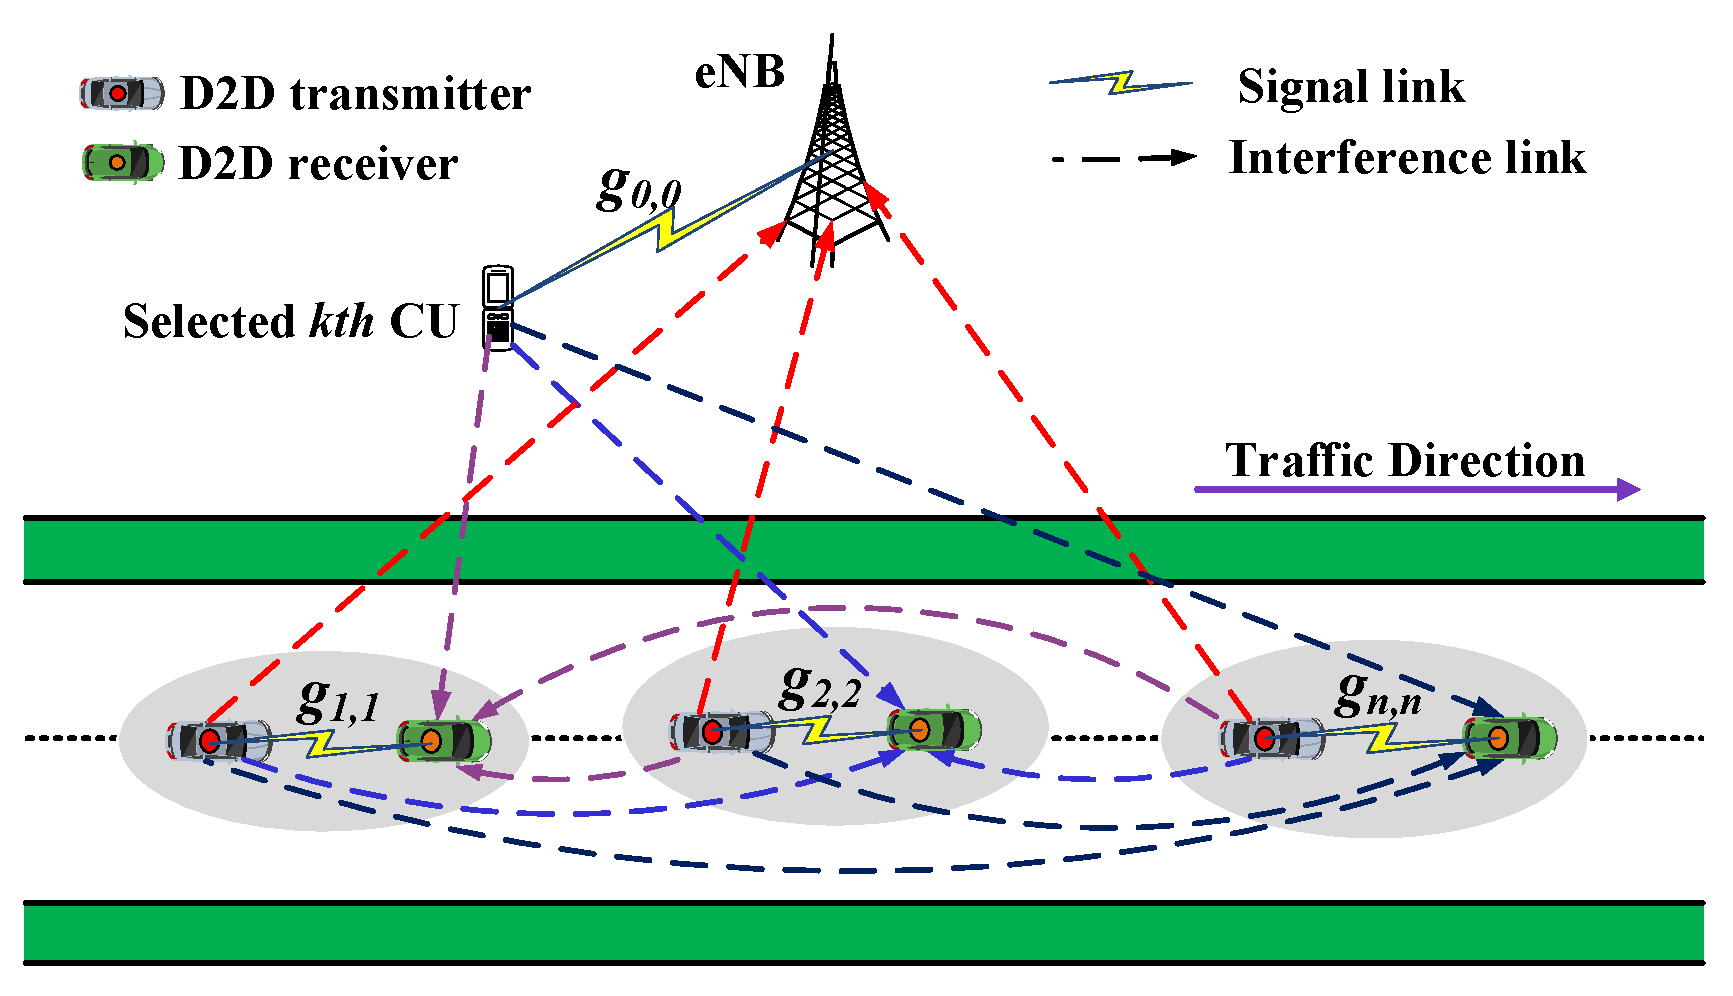
\includegraphics[width=8cm]{1.eps}
\caption{system model.}
\end{figure}

\begin{figure}[h]
\centering
%\hspace{1.0cm}
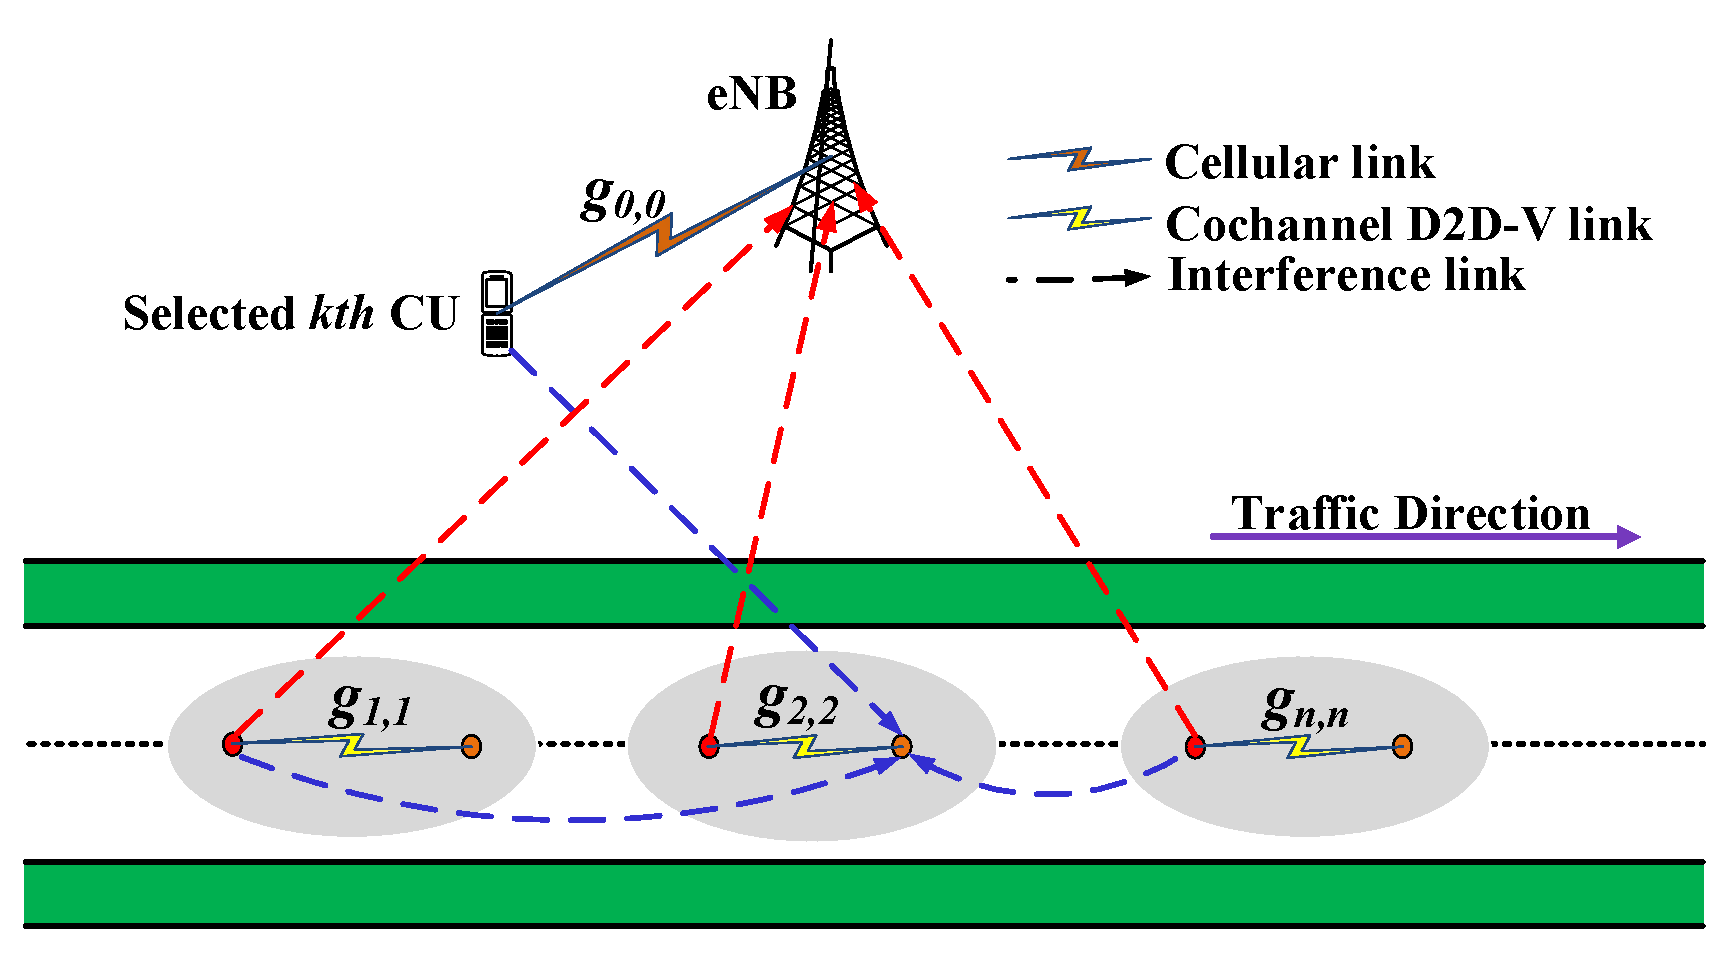
\includegraphics[width=8cm]{2.eps}
\caption{simplified system model.}
\end{figure}

In Fig. 1 and Fig. 2, the eNB is clearly marked, and other weaknesses of drawing have also been improved. The ``n" means the $n_{th}$ D2D-V pairs. This model has good network scalability, firstly, multiple D2D pairs can simultaneously reuse the uplink communication channel of a CU. Secondly, different CUs use different frequencies for communication, so multiple CUs can provide reusable spectrum resources for a large number of vehicle users at the same time. When there are vehicles coming in and out, round channel selection fashion can achieve effective user access and elimination [1]. Therefore, this model can be extended to more dense vehicle scenarios, coupled with effective vehicle access and elimination, so that the scalability of the network can be achieved.

\footnotesize
[1] Y. Ren, F. Liu, Z. Liu, C. Wang, and Y. Ji, ``Power control in D2D-based vehicular communication networks," \emph{IEEE Trans. Veh. Technol.}, vol. 64, no. 12, pp. 5547-5562, Oct.
\normalsize


%R2Q4
\item\textbf{Question}: There is no explanation for ``CU-I",``V2I link", ``CU-V", and ``V2V",especially for ``I". This will make reader who have no communication foundation confused.

    \textbf{Answer}: Thanks for the reviewer's carefulness! The related work has been presented as follows and marked {\color{red} in red} in the paper. {\color{red} There are five kinds of links in the vehicular two-tier networks: CU-I link (the transmitter is CU and the receiver is the eNB), V2I link (the transmitter is vehicle user and the receiver is the eNB), CU-V link (the transmitter is cellular user and the receiver is the vehicle user), vehicle-to-vehicle (V2V) signal link, and V2V interference link.}

%R2Q5
\item\textbf{Question}: The Bernstein approximation and exponential integration methods are used to transform the uncertain probability constraints into a certainty form. However, the motivations are suggested to give clearly. For instance, why does not the uniform method such as integral transformation convert the probability constraint?

    \textbf{Answer}: Thanks for the reviewer's comment! In this article, the two converting ways (the Bernstein approximation and integral methods) have different application conditions, and we can not combine them or develop only one way to simplify the analysis. The Bernstein approximation method is adopted to deal with the interference constraint with channel uncertainty. However, traditional methods are useless to express the interference constraint into a closed form. To obtain the closed form, Nemirovski and Shapiro have proposed a convex approximation approach in [1]. Therein, the Bernstein approximation method has commonly been used to approximate the chance constraint [2], [3]. Since the same limitations of multiple-variable coupling and channel uncertainty, the Bernstein approximation method is used in this paper. Different from the complex interference constraint, the delivery rate and delay constraints can get the closed form by exponential integration. Furthermore, the exact solutions are available, so the integral methods are used.

To sum up, the interference constraints with multiple-variable coupling and channel uncertainty are difficult to obtain the closed form and exact solutions, so the Bernstein approximation method is used to simplify the constraints and get sub-optimal solutions. In contrast, the delivery rate and delay constraints are easier to handle, and the integral methods can obtain the optimal solutions.

\footnotesize
[2] A. Nemirovski and A. Shapiro, ``Convex approximations of chance constrained programs," \emph{SIAM J. Optim.}, vol. 17, no. 4, pp. 969-996, 2006.

[3] S. Wang, W. Shi, and C. Wang, ``Energy-efficient resource management in OFDM-based cognitive radio networks under channel uncertainty," \emph{IEEE Trans. Commun.}, vol. 63, no. 9, pp. 3092-3102, Sep. 2015.

[4] N. Soltani, S. Kim, and G. Giannakis, ``Chance-constrained optimization of OFDMA cognitive radio uplinks," \emph{IEEE Trans. Wireless Commun.}, vol. 12, no. 3, pp. 1098-1107, Mar. 2013.
\normalsize


%R2Q6
\item\textbf{Question}: The pricing scheme is introduced in the proposed framework, however, the definition and the physical meaning of the price should be given. Moreover, the pricing or bargaining process should also be stated clearly.
    
    \textbf{Answer}: Thanks for the reviewer's valuable comment! We want to explain this and hope to get your approval. In wireless communication, interference is regarded as an allocatable resource. In the upper network, the eNB prices the interference, and charges from D2D-V users as its profit. In the lower subgame, the utility function is the difference between the D2D-V users' sum transmission rates and the cost of purchasing interference. When the power of a D2D-V user increases, the sum transmission rate will increase. However, more interference will follow, and the lower network needs to spend more interference cost, which is the $punishment$ from the upper network. From a mathematical point of view, price is a weighting coefficient. From a physical point of view, the price describes the interest relationship between the upper and lower layers of the network. The price-penalty mechanism is the same as the power control project, which is to achieve the purpose of optimizing communication performance by formulating corresponding pricing strategies.
    
%R2Q7
\item\textbf{Question}: Only the simple scenario, one CU and four clusters, is simulated in the simulation. However, when the vehicle density is large, can the proposed algorithm guarantee good communication performance?
    
    \textbf{Answer}: Thanks for the reviewer's comment! As explained in question 3, the D2D-V communication model is suitable for dense vehicle scenarios. Firstly, multiple D2D pairs can simultaneously reuse the uplink communication channel of a CU. Secondly, different CUs use different frequencies for communication, so multiple CUs can provide reusable spectrum resources for a large number of vehicle users at the same time. In the simulation, we have verified the robustness of the system and the effectiveness of the interference management mechanism. Such a scenario (one CU and four clusters) is not a special case, but a representative display. When the density of vehicles increases, the biggest challenge is that multi-user interference will increase accordingly. The proposed interference management mechanism based on probability constraints can deal with it well and ensure the robust and reliable vehicular communications.

%R2Q8
\item\textbf{Question}: There are some typos and errors in the manuscript, please polish the whole paper carefully.

    \textbf{Answer}: Thanks for the reviewer's carefulness and sorry for our inaccurate statements! We have checked and corrected the manuscript carefully to avoid any errors and typos. The modifications are marked in red.
   
   
\end{enumerate}

Finally, the authors thank the reviewer for the provided comments, and the time and efforts he/she has spent in the review again. Without these careful comments, the paper would not reach its current quality. We hope that the above modifications have answered the reviewer's concerns. We will happily welcome any additional suggestions and feedback from the reviewer.

\newpage

{\Large \underline{Response to Reviewer 3}}

We would like to thank the reviewer for spending his/her time to assess the paper, and make very constructive and detailed informative comments provided in the review. Our responses are given as follows:

\begin{enumerate}
%R3Q1
\item
\textbf{Question}: Two channel models are considered in the manuscript to describe the low mobility link and high mobility link, however, the channel power gains are affected by many factors. Why only the Doppler effect is considered? Please clarify.

\textbf{Answer}: Thanks for the reviewer's comment! We would like to clarify that not only the Doppler effect but also other features are considered to describe the channel states. In the practical D2D-V communication environments, large-scale slow fading and small-scale fast fading are both existent and can not be ignored. Large-scale slow fading includes path loss and shadow fading. Besides, due to the movement of vehicles, the small-scale fast fading is mainly caused by the Doppler effect. Therefore, both path loss, shadow fading, and the Doppler effect are considered to describe time-varying and uncertain channels accurately.

For example,
\begin{eqnarray}
&g_{i,j}=\left\{
\begin{array}{lll}
     S_{i,i}^{k}|\eta_{i,i}^{k}|^{2},\quad i=j,\\
     S_{i,j}^{k}(\vartheta_{i,j}^{k}\hat{\eta}_{i,j}^{k})^{2}+S_{i,j}^{k}(\epsilon_{i,j}^{k})^{2},\quad i\neq j,\
\end{array}
\right.
\end{eqnarray}
\begin{eqnarray}
S_{i,i}^{k}=L_{i,i}^{k}(d_{i,i}^{k})^{-\alpha_i},           &i\in \mathcal{I},
\end{eqnarray}
where $S_{i,i}^{k}$ is large-scale slow fading, which includes path loss $(d_{i,i}^{k})^{-\alpha_i}$ and shadow fading $L_{i,i}^{k}$. In the low mobility links, the small-scale fast fading is formulated as $|\eta_{i,i}^{k}|^{2}$. However, the vehicle movement is considered in the high mobility links, the first-order Markov process $\eta=\vartheta\hat{\eta}+\epsilon$ is introduced and the small-scale fast fading is formulated as $(\vartheta_{i,j}^{k}\hat{\eta}_{i,j}^{k})^{2}+(\epsilon_{i,j}^{k})^{2}$.


%R3Q2
\item \textbf{Question}: According to the Theorem 3, there is a precondition to approach the GE. I wonder that if the condition can not be satisfied, how can the users allocate the power? My question is not casual as the channel conditions are changing, the precondition will not hold all the time.
    
\textbf{Answer}: Thanks for the reviewer's valuable comment! We recognize that the establishment of Theorem 3 is based on this precondition $g_{i,i}^- >\sum\limits_{j=0,j\neq i}^N g_{j,i}^+$. The precondition is universally established, which is also assumed and applied by the article [1]. However, the considerations raised by the reviewers are also possible. When the channel gain of some interference links is too large, Theorem 3 is invalid. Therefore, to make the algorithm of this paper more applicable, some prerequisite work needs to be prepared. When a small probability event with excessive interference gain occurs, related tasks such as user elimination can be used reasonably to meet this precondition [2].

\footnotesize
[1] Z. Liu, W. Wang, K. Chan, et al, ``Rate Maximization for Hybrid Access Femtocell Networks with Outage Constraints Based on Pricing Incentive Mechanism," \emph{IEEE Trans. Veh. Technol.}, vol. 69, no. 6, pp. 6699-6708, Apr. 2020.

[2] S. Wang, R. Ruby, V. Leung, et al, ``A Low-Complexity Power Allocation Strategy to Minimize Sum-Source-Power for Multi-User Single-AF-Relay Networks," \emph{IEEE Transactions on Communications}, vol. 64, no. 8, pp. 3275-3283, Aug. 2016.
\normalsize

%R3Q3
\item \textbf{Question}: As for the delay and delivery rate constraints, it is unclear that how to get the relationship between the constraints and the optimization variables. Moreover, there are several parameters introduced in the formulas (13) and (14), more discussions about them are needed, such as how to choose them, are there effect on the optimal solutions?

\textbf{Answer}: Thanks for reviewer's valuable comment! We use Lagrangian multiplier method to deal with game problems containing the delay and delivery rate constraints.
\begin{equation}
\begin{array}{*{20}{ll}}
 \!\!\nu_{i}^{(t+1)}\!\!=\!\![\nu_{i}^{(t)}\!\!+\!K_{\nu}^{(t)}(\frac{(1-\varsigma_i D_{i,\textrm{max}})(I_{th}+\delta^2)}{\tau_i D_{i,\textrm{max}}\ln(1-\varepsilon_2)}-p_i \bar{g}_{i,i})
]^+\!,
\end{array}
\end{equation}
\begin{equation}
\begin{array}{*{20}{ll}}
 \!\!\varphi_{i}^{(t+1)}\!\!=\!\![\varphi_{i}^{(t)}\!\!+\!K_{\varphi}^{(t)}(\frac{\gamma_{th}
 (I_{th}+\delta^2)}{\ln\Omega_{i,\textrm{min}}\ln(1-\varepsilon_3)}-p_i \bar{g}_{i,i})
]^+\!,
\end{array}
\end{equation} 
\begin{eqnarray}
 \begin{array}{lll}
&\!\!\!\!\!\!\!\!\frac{\partial\textit{L}_i(\mathbf{p}:\bm{\mu},\bm{\lambda},\bm{\nu},\bm{\varphi})}{\partial p_i}\!\!=\!\!\frac{W g_{i,i}^-\epsilon_{i,i}}{p_i g_{i,i}^- +I_i(p_{-i})+\delta^2}-c_i g_{i,0}^+\\
&-\!\!\!\!\sum\limits_{j=0,j\neq i}^N (\mu_{j}\eta_{i,j}\!+\!\lambda_{i,j}\sqrt{N}\sigma_{i,j}\alpha_{i,j})+\nu_i \bar{g}_{i,i}+\varphi_i \bar{g}_{i,i} \\
\end{array}
\end{eqnarray}

Let $\frac{\partial\textit{L}_i(\mathbf{p}:\bm{\mu},\bm{\lambda},\bm{\nu},\bm{\varphi})}{\partial p_i}=0$,
the optimal power is:
\begin{equation}\label{43}
\begin{array}{*{20}{ll}}
 p_i^{*}=\frac{W}{c_i g_{i,0}^+ + \Pi_i^{*}}-\frac{I_i^{*}(p_{-i})+\delta^2}{g_{i,i}^-}
\end{array}
\end{equation}

It can be seen that the constraints and optimization variables are connected through the iterative Lagrangian multipliers. When we change the constraint parameters, the iteration Lagrangian multipliers will change, and the optimization variables will also change accordingly. As for the selection of parameters, we have to determine according to actual standards and target requirements. For example, the process of a packet arriving at the D2D receiver is a Poisson process with parameter $\varsigma$, the length of the data packet obeys the exponential distribution of parameter $\tau$, and choose the packet delivery rate threshold $\Omega_{i,\textrm{min}}$ and delay threshold $D_{i,\textrm{max}}$ according to our requirements.

%R3Q4
\item \textbf{Question}: In table I, the index sets $I$ and $J$ are same, please check.

\textbf{Answer}: Thanks for reviewer's comment! After checking, there is no errors in table I. $\mathcal{I}$=$\{0,1,\cdots,i,\cdots,N\}$, $\mathcal{J}$=$\{0,1,\cdots,j,\cdots,N\}$ are used to represent vehicle receiving and sending collections, respectively.

%R3Q5
\item \textbf{Question}: There are too many notations and symbols are introduced when introducing Bernstein approximation of the interference constraints in section III, it is confusing and difficult to follow. If the results come from existing conclusion, it is better to quote the reference and reduce the expressions. If not, please move it to the appendix.

\textbf{Answer}: Thanks for reviewer's valuable suggestions! To make the article clear, this part of the approximate transformation work is transferred to ``Appendix A". In the text, it is presented as follows
{\color{red}\begin{theorem}
The interference constraint of all cochannel D2D-V links $\textrm{Pr}\left\{I_{j} \leq I_{th}\right\}\geq1-\varepsilon_1,\quad  i\in\mathcal{I}, j\in\mathcal{J}$ is reformulated as the separable constraints (\ref{27}) and (\ref{28}). The auxiliary variables $\bm{\Theta}$ is introduced into the new separation structure, which is express as $\Theta_{i,j}$$=$$\sigma_{i,j}\alpha_{i,j} p_i$.
\begin{eqnarray}\label{27}
 \begin{array}{lll}
\sum\limits_{i=0,i \neq j}^{N}\eta_{i,j}p_i+\sqrt{2\ln(\frac{1}{\varepsilon})}\sum\limits_{i=0,i \neq j}^{N}\Theta_{i,j} \leq I_{th},
\end{array}
\end{eqnarray}
\begin{eqnarray}\label{28}
 \begin{array}{lll}
\sqrt{N}\sigma_{i,j}\alpha_{i,j} p_i\leq \sum\limits_{i^{'}=0,i^{'}\neq j}^{N}\Theta_{i^{'},j},\quad \forall j\in\mathcal{J},i\in\mathcal{I}.
\end{array}
\end{eqnarray}
\end{theorem}

where $\eta_{i,j}=\hat{g}_{i,j}+\phi_{i,j}^{+}\alpha_{i,j}+\beta_{i,j}$, $\phi_{i,j}^{+}$ and $\sigma_{i,j}$ are constants which are determined by the given families of the probability distributions. $-1$$\leq$$\phi_{i,j}^{+}$$\leq$$1$, $\sigma_{i,j}$$\geq$$0$. [3] shows how the values of $\phi_{i,j}^{+}$ and $\sigma_{i,j}$ are obtained. The distributions of $\tilde{g}_{i,j}$ are assumed to be bounded by $[a_{i,j}, b_{i,j}]$, and the constants $\alpha_{i,j}$$=$$\frac{1}{2}(b_{i,j}$$-$$a_{i,j})$$\neq$$0$ and $\beta_{i,j}$$=$$\frac{1}{2}(b_{i,j}$$+$$a_{i,j})$ are used to normalize the supports within the range of $[-1, 1]$.

\emph{Proof:} See Appendix A}

\footnotesize
[3] Y. Xie, Z. Liu, K. Chan, et al, ``Energy-Spectral Efficiency Optimization in Vehicular Communications: Joint Clustering and Pricing-Based Robust Power Control Approach," \emph{IEEE Trans. Veh. Technol.}, vol. 69, no. 11, pp. 13673-13685, Sep. 2020.

\normalsize

%R3Q6
\item \textbf{Question}:In the simulation part, figure 3 and 4 are the power levels of cellular user and D2D user, they can be combined. The legends in figure 7, figure 8 and figure 9 are missed. In figure 14, the legend should be $U_{sum}$.

\textbf{Answer}: Thanks for reviewer's carefulness and valuable suggestions! We combine fig.3 and 4, a new figure which names ``Power convergence performance of CU and D2D-V users" is shown.

\begin{figure}[htbp]
\centerline{\includegraphics[width=6cm]{3.eps}}
\center{\footnotesize Fig. 3 Power convergence performance of CU and D2D-V users.}
\end{figure}
The legends in figure 7, figure 8, and figure 9 are listed, the newly changed picture is shown in fig.6, 7, and 8. As for figure 14, the legend is modified to $U_{sum}$, and the modified simulation diagram fig.13.

\begin{figure}[htbp]
\centerline{\includegraphics[width=6cm]{6.eps}}
\center{\footnotesize Fig. 6 Outage probability comparison of interference constraints.}
\end{figure}
\begin{figure}[htbp]
\centerline{\includegraphics[width=6cm]{7.eps}}
\center{\footnotesize Fig. 7 Outage probability comparison of delay constraints.}
\end{figure}
\begin{figure}[htbp]
\centerline{\includegraphics[width=6cm]{8.eps}}
\center{\footnotesize Fig. 8 Outage probability comparison of delivery rate constraints.}
\end{figure}
\begin{figure}[htbp]
\centerline{\includegraphics[width=6cm]{13.eps}}
\center{\footnotesize Fig. 13 Utility value versus vehicle speed.}
\end{figure}

%R3Q7
\item \textbf{Question}:The contributions should be refined to highlight the difference and novelty compared with existing works. And also the more relevant references on the price reward and punishment mechanism are suggested to review, because the Price-Penalty is one of motivations in this paper to get the optimal power allocation.

\textbf{Answer}: Thanks for the reviewer's valuable comment! To form a better work, the Contributions were rewritten carefully and meticulously. The modifications are marked in red.

{\color{red}\begin{itemize}
    \item A more practical and dynamic communication scenario is considered, and the channel uncertainty is highlighted in the vehicular networks. Instead of the impractical assumption that the perfect or known CSI is available, the first-order Gauss-Markov process is introduced to describe the imperfect channel gains. In particular, vehicle mobility is considered to simulate time-varying fast fading, which is the main factor of channel uncertainty.
    \item More efficient many-to-one reusing mode is adopted to improve spectrum utilization. From the perspective of robust transmission, the probability constraint is constructed to depress the uncertain co-channel interference. To accommodate the probability constraint with multiple-variable coupling, the Bernstein approximation method is used to transform it into a solvable closed form. Particularly, different from the previous protection of a single CU, the Bernstein method is successfully extended to deal with multiple D2D-V users' interference constraints.
    \item To realize joint optimization of the upper and lower networks, a price-penalty mechanism is novelly proposed to cooperate with the power control scheme. Outperform the pure power control, the beneficial relationships are highlighted. For selfish players, unilateral strategy adjustment brings bigger self-interest, but at the expense of others. By charging for interference, the price-penalty mechanism limit the selfish behaviors and balance the benefits of all parties. Finally, a robust Stackelberg game framework is constructed to realize cross-layer resource allocation, which is based on the price-penalty mechanism and power control scheme.
\end{itemize}}

More detailed content and relevant references about the price penalty mechanism are introduced in the paper. In wireless communication, interference is regarded as an allocatable resource [4]. In the upper network, the eNB prices the interference, and charges from D2D-V users as its profit. In the lower subgame, the utility function is the difference between the D2D-V users' sum transmission rates and the cost of purchasing interference. When the power of a D2D-V user increases, the sum transmission rate will increase. However, more interference will follow, and the lower network needs to spend more interference cost, which is the $punishment$ from the upper network [5]. From a mathematical point of view, price is a weighting coefficient. From a physical point of view, the price describes the interest relationship between the upper and lower layers of the network. The price-penalty mechanism is the same as the power control project, which is to achieve the purpose of optimizing communication performance by formulating corresponding pricing strategies.

\footnotesize
[4] Y. Xie, Z. Liu, K. Chan, et al, ``Energy-Spectral Efficiency Optimization in Vehicular Communications: Joint Clustering and Pricing-Based Robust Power Control Approach," \emph{IEEE Trans. Veh. Technol.}, vol. 69, no. 11, pp. 13673 - 13685, Sep. 2020.

[5] K. Xin, Z. Rui, M. Motani, ``Price-based resource allocation for spectrum-sharing
femtocell networks: a stackelberg game approach," \emph{IEEE J. Sel. Areas Commun.}, vol. 30, no. 3, pp. 538-549, Mar. 2012.
\normalsize


\end{enumerate}

Finally, the authors thank the reviewer for the comments provided, and the time and efforts the reviewer has spent in the review again. Without these careful comments, the paper would not reach its current quality. We hope that the above modifications have answered the reviewer's concerns. We look forward to hearing from you regarding our submission. We would be glad to respond to any further questions and comments that you may have.

\newpage

{\Large \underline{Response to Reviewer 4}}

We would like to thank the reviewer for spending his/her time to assess the paper, and make very constructive and detailed informative comments provided in the review. Our responses are given as follows:

\begin{enumerate}
%R4Q1
\item
\textbf{Question}: In the section of Related Works, the connection between paragraphs should be strengthened to form a closer work.

\textbf{Answer}: Thanks for the reviewer's comment! To form a closer work, the Related Works were rewritten carefully and meticulously, and the connection between paragraphs is strengthened. The modifications are marked in red.


%R4Q2
\item \textbf{Question}: Clear definition and notations are needed. In the Notations, $\Upsilon$ is the parameter of exponential distribution. However, it appears twice in this paper. Besides, the Euclidean space $R^N$ should be added to the Notations.

\textbf{Answer}: Thanks for the reviewer's comment! Clear definition and notations are finished and shown as follows
\begin{table}[!h]
\caption{Notations}\label{tab1}
\centering
{\small\begin{tabular}{ll}
\hline
\hline
$\mathcal{I}$  & The index set $\mathcal{I}$=$\{0,1,\cdots,i,\cdots,N\}$\\
$\mathcal{J}$   & The index set $\mathcal{J}$=$\{0,1,\cdots,j,\cdots,N\}$\\
$\textrm{Pr}\{\cdot\}$ & Probability function \\
$\Upsilon$   & Parameter of exponential distribution \\
$E\{\cdot\}$   & Exponential distribution \\
$\mathbb{R}^N$      & Set of $N$-dimensional real vectors\\
$\mathcal{R}^N$   & Euclidean space\\
$\mathbb{E}\{\cdot\}$   & Mathematical expectation of a random variable \\
\hline
\hline
\end{tabular}}
\end{table}

%R4Q3
\item \textbf{Question}: To find the optimal solution of the upper subproblem P2, the original objective function is transformed. When the interference term is regarded as a constant value, it seems that the transformation is only a simple logarithmic transformation and has little significance. So I think this transformation is redundant.

\textbf{Answer}: Thanks for the reviewer's comment! To express the objective function more clearly and facilitate the process of derivation, the following conversion is completed.
\begin{eqnarray}
U_{\textrm{sum}}\!\!=\!\!\sum\limits_{i=1}^N \big[ W\log(1+\bar{\gamma}_{i}(\mathbf{p}))\!\!-c_{i} p_i g_{i,0}\big]
\end{eqnarray}

According to $\log(a\div b)=\log(a)-\log(b)$,
\begin{equation}
U_{\textrm{sum}}=f(p)-h(p)-\sum_{i=1}^N c_{i}p_i g_{i,0}^+,
\end{equation}
\begin{equation}
f(p)=\sum_{i=1}^N W\log\big(p_i g_{i,i}^- +I_i(p_{-i})+\delta^2\big),
\end{equation}
\begin{equation}
h(p)=\sum_{i=1}^N W\log\big(I_i(p_{-i})+\delta^2\big),
\end{equation}
where $I_i(p_{-i})=\sum_{j=0,j\neq i}^N p_j g_{j,i}$.

%R4Q4
\item \textbf{Question}: The research is under channel uncertainty, multi-user interference, and a high-speed environment. For the vehicular movement characteristics, there are relevant contents in the simulation, but I don't understand how the vehicle speed affects the system performance.

\textbf{Answer}: Thanks for the reviewer's valuable comment! The impact of the vehicle movement on the network is reflected in the channel. In a high mobility communication link, the movement of vehicles will bring a Doppler shift, which in turn leads to uncertainty in the channel state. To accurately describe the channel state, we introduce a first-order Markov model which considers the speed.
\begin{eqnarray}
\eta=\vartheta\hat{\eta}+\epsilon,
\end{eqnarray}
\begin{eqnarray}
\vartheta = J_0(2\pi{f_d}T),
\end{eqnarray}
\begin{eqnarray}
f_d=\upsilon{f_c}/c,
\end{eqnarray}

To verify the impact of vehicle speed on system performance, Fig.13 is shown when different vehicle speeds are simulated. It can be seen from Fig. 13 that with the increase of vehicle speed, the utility value of the lower network decreases, whereas the utility value of the upper network increases. This is because the higher speed will cause a greater Doppler frequency shift in the lower network, increase channel uncertainty, and make the signal link suffer more serious interference. Therefore, the utility of the lower network reduces, and the upper network that charges for the interference will obtain a better utility.

\begin{figure}[htbp]
\centerline{\includegraphics[width=6cm]{13.eps}}
\center{\footnotesize Fig. 13 Utility value versus vehicle speed.}
\end{figure}

%R4Q5
\item \textbf{Question}: Eq. (27), (28), and (29) are the theoretical basis of Bernstein approximation. However, what does $\rho$ mean in Eq. (28)? There is no clear explanation.

\textbf{Answer}: Thanks for the reviewer's carefulness and valuable comment! The Bernstein approximation method is well organized in [1]. However, this paper also didn't name $\rho$. According to [1],
\begin{eqnarray}
\textrm{Pr}\left\{f_0(\mathbf{p})+\sum\limits_{n=1}^{N}\eta_nf_n(\mathbf{p}) \leq 0 \right\}\geq1-\varepsilon,
\end{eqnarray}

When the following conditions hold, 

a) $\{f_n(\mathbf{p})\}$ are affine in $\mathbf{p}$;

b) $\{\eta_n\}$ are independent of each other;

c) $\{\xi_n\}$ share the bounded support of [-1,1], which is in the range of $-1\leq\xi_n\leq 1,\forall n = 1, 2,\cdot \cdot \cdot, N$.

For any $\rho>0$, a conservative approximation substitute is as follows,
\begin{eqnarray}
\inf\limits_{\rho>0}\left[f_0(\mathbf{p})+\rho\sum\limits_{n=1}^{N}\Omega_n(\rho^{-1}f_n(\mathbf{p}))+\rho \ln(\frac{1}{\varepsilon})\right]\leq0,
\end{eqnarray}

Therefore, the $\rho$ is just a parameter, we name it the ``conservative approximate parameter" in the Bernstein approximation method.

\footnotesize
[1] A. Nemirovski and A. Shapiro, ``Convex approximations of chance constrained programs," \emph{SIAM J. Optim.}, vol. 17, no. 4, pp. 969-996, 2006.
\normalsize

%R4Q6
\item \textbf{Question}: Convergence performance is demonstrated in Fig.3, 4, 5, and 6. In my opinion, the optimal variables should be with the same convergence performance. It seems that the power of vehicles, prices, and utilities are with lower convergence than the power of CU. Why?

\textbf{Answer}: Thanks for the reviewer's carefulness and valuable comment! According to these pictures, the convergence of CU's power iteration seems to be faster than the convergence of vehicles' power iteration, price, and utility. However, they all reach convergence in the tenth step at the same time. Hence, the power of vehicles, prices, and utilities are with the same convergence performance as the power of CU. In the step1-step5, both of the variables change greatly. Compared with vehicles' power, the changes of CU's power, price, and utility are much smaller in step5-step10. The situation is reasonable. When the game is repeated, some variables will approach the equilibrium solution of the game in advance, and some variables will be a little slower, and eventually, they will reach the game equilibrium solution at the same time.

%R4Q7
\item \textbf{Question}: In the Simulation, Fig. 12 shows the comparison of actual outage probability of different papers with the parameters $\varepsilon_1$=$\varepsilon_2$=$\varepsilon_3$=0.1. Why is it 0.1? Can this conclusion be successful for other values?

\textbf{Answer}: Thanks for the reviewer's carefulness and valuable comment! Fig. 11 (Modified simulation diagram number) shows the comparison of actual outage probability of different papers. As a representative, the conclusion is shown when the parameters $\varepsilon_1 =\varepsilon_2=\varepsilon_3=0.1$. It is emphasized that when this parameter is selected as other values, the following conclusions are still coincident.

%R4Q8
\item \textbf{Question}: There are some drawing problems in the simulation figures.

- The width of the line in Fig.3, 4, 5, and 6 is different from it in Fig.7, 8, 9, and 11.

- In Fig.10, the description of $\varepsilon_1$, $\varepsilon_2$, and $\varepsilon_3$ are confused. Besides, this figure aims to show the utility values of the lower network versus outage probability 0.1,0.2,0.3, and 0.4. So it is better to remove the intermediate ticks (0.05, 0.15, 0.25, and 0.35).

- In Fig. 12, 1, 2, 3, and 4 represent four D2D-V users, respectively. However, 1, 2, 3, and 4 represent the four methods "Stackelberg game with imperfect CSI," "The SCA", "Stackelberg game with perfect CSI" and "The D.C. program." The description is conflicting and needs to be adjusted.

\textbf{Answer}: Thanks for the reviewer's carefulness. The drawing problems in the simulation figures have been checked and corrected carefully.

- The width of the line is unified. Besides we combine fig.3 and 4, a new figure which names ``Power convergence performance of CU and D2D-V users" is shown.

\begin{figure}[htbp]
\centerline{\includegraphics[width=6cm]{3.eps}}
\center{\footnotesize Fig. 3 Power convergence performance of CU and D2D-V users.}
\end{figure}

- The newly changed picture is shown in fig.9.
\begin{figure}[htbp]
\centerline{\includegraphics[width=6cm]{9.eps}}
\center{\footnotesize Fig. 9 Utility value of the lower network versus target outage probability threshold $\varepsilon_1$, $\varepsilon_2$, or $\varepsilon_3$ .}
\end{figure}

- For the third point, we want to explain this and hope to get your approval. In the abscissa of Fig. 11, 0, 1, 2, 3, 4 represent the CU and the vehicle user. In the abscissa of Figure 12, 1, 2, 3, 4 represent four different methods. They have no actual meaning and are just number representatives.

%R4Q9
\item \textbf{Question}:Some typos and minor concerns:

- The formation of section titles is not unified.

-Introduction: Second, ..., but fail to the spectrum utilization. fail to-- fail in.

-Section II. A: the period for D2D-V transmitters or CU broadcasting their CSI, ``broadcasting" -- ``to broadcast".

-Section III.B: ``Transformations of the Lower Subgame" appears twice. The first should be ``Transformation of Upper Subgame". The second should be ``Transformation of Lower Subgame".

\textbf{Answer}: Thanks for the reviewer's carefulness. We are sorry for the negligence! We have checked these parties carefully, the corresponding typos and minor concerns have been revised in the revision. The modifications are marked in red.

\end{enumerate}

Finally, the authors thank the reviewer for the comments provided, and the time and efforts the reviewer has spent in the review again. Without these careful comments, the paper would not reach its current quality. We hope that the above modifications have answered the reviewer's concerns. We look forward to hearing from you regarding our submission. We would be glad to respond to any further questions and comments that you may have.


\end{document}
